\documentclass[lettersize,journal]{IEEEtran}
\usepackage{amsmath,amssymb}
\usepackage{fontspec}
\setmainfont{texgyretermes}[Extension=.otf,UprightFont=*-regular,BoldFont=*-bold,ItalicFont=*-italic,BoldItalicFont=*-bolditalic]
\usepackage[warnings-off={mathtools-colon,mathtools-overbracket}]{unicode-math}
\setmathfont{texgyretermes-math.otf}
\usepackage{array,booktabs,tabularx,longtable}
\usepackage{graphicx}
\usepackage{url}
\usepackage[hidelinks]{hyperref}
\usepackage{xcolor}
\usepackage{fancyhdr}
\renewcommand{\tabularxcolumn}[1]{p{#1}}
\setlength{\tabcolsep}{3pt}
\emergencystretch=2em
% Generated by paper4/manuscript/build.py from paper4/paper/*.md: edit the Markdown, not this file.

\begin{document}
\title{What a Traffic Sensor Buys: No Forecastable Spatial Signal Beyond the Calendar on Uninstrumented Segments, and What a Loop Detector Measures of Congestion}
\author{Draft of the internal review, 2026-11-08. Authors to be confirmed.%
\thanks{Full draft typeset from \texttt{paper4/paper/*.md} by \texttt{paper4/manuscript/build.py}. Every number is checked against the frozen records by \texttt{paper4/analysis/main.py}. Citations are marked [key] or [ref:~\ldots] where a reference is still to be chosen.}}
\markboth{Paper 4 --- full draft for the internal review}{Paper 4 --- full draft}
\maketitle
\begin{abstract}
A road operator pays for each traffic sensor and covers only part of the network. We ask what sensors buy for the segments that have none, and what the most common urban sensor measures. On three cities of the Traffic4cast benchmark (Madrid, London, Melbourne), we forecast congestion in three classes 15–120 minutes ahead on segments the model never sees. A graph model gains nothing over the same model without its graph, at any spacing from 43 to 397 m and any coverage from 10\% to 60\%. The labels of nearby segments agree within about 250 m, but calibrated, that agreement stays 1–3 points below the model without spatial exchange, and net of the hour of the week it adds nothing. Placement changes how many uncovered segments lie near a sensor, not how well they are forecast. Against independent speed references in Madrid and Austin, a loop detector detects congestion (area under the curve 0.984) but ranks its level poorly (rank correlation +0.249); matching loops to road segments accounts for about half of their disagreement with probe speeds on arterials; and aggregating lanes hides episodes on one lane. Every experiment was pre-registered and frozen, and one script regenerates every number.
\end{abstract}
\begin{IEEEkeywords}
Traffic forecasting, graph neural networks, sensor placement, kriging, loop detectors, congestion detection, pre-registration.
\end{IEEEkeywords}

% ---- section_introduction.md (10e7fb77296ecb1a)
\section{Introduction}
A road operator who installs traffic sensors pays for each one, and covers only part of the network. Two decisions follow:

\begin{itemize}
\item what each sensor should measure;
\item how many sensors to install, and where.
\end{itemize}

For the second decision, the usual hope is that instrumented segments inform the segments without a sensor. Spatio-temporal graph models propagate information along the road network [wu2019gwnet], and kriging methods estimate unobserved locations from observed ones [wu2021ignnk]. If that propagation works, coverage and placement buy accuracy on the whole network, not only where the sensors are.

We test that hope on one task: classifying congestion in three classes (free flow, slowed, congested) at 15–120 minutes ahead, on segments that have no sensor. A segment without a sensor is never seen by the model: it is not in the input, in the training loss, in the normalisation or in the class weights. This is the operator's situation, and it is stricter than the evaluation of a deliverable that preceded this work, where the segments said to be hidden were training targets.

The data are the measured speeds of three cities from the Traffic4cast benchmark (Madrid, London and Melbourne, 828, 774 and 587 segments) [ref: Traffic4cast 2022]. The forecast is scored by weighted cross-entropy, which we abbreviate as wCE: the cross-entropy of the predicted class probabilities, with class weights that give the rare congested class the same total weight as the others.

The reference is a model without spatial exchange. It is the same temporal network as the graph model, Graph WaveNet [wu2019gwnet], with its graph removed. It forecasts a segment from the calendar it has learned, since the segment's own data never reach it.

Against that reference we ask whether instrumented neighbours help, in four ways:

\begin{itemize}
\item with a learned graph model, varying the spacing of the network and the instrumented fraction;
\item with predictors that need no training, which read the neighbours' labels directly;
\item with those labels calibrated on the instrumented segments, with and without the calendar;
\item by measuring how close each placement rule brings the uncovered segments to a sensor.
\end{itemize}

For the first decision, we ask what the most common urban sensor, the loop detector, measures of congestion. Three datasets give a speed reference independent of the loop's reconstruction: the M30 ring of Madrid, where the same device measures speed; the Madrid arterials, where loops are matched to probe speeds; and Austin, with radar detectors per lane.

Every experiment was pre-registered before any test metric was computed, under the method of an earlier study by the same authors [ref: Paper 1]: signed pre-registrations, frozen records generated by script, intervals from a joint resample of seeds and blocks of the network, and two reading scales (the sign of the interval and a margin of 3\% of the reference wCE).

We address four research questions.

\begin{itemize}
\item \textbf{RQ1 (what to measure).} Against an independent speed reference, what does a loop detector measure of congestion: its level, its occurrence, or both? How much of the disagreement on urban arterials is due to the spatial matching of loops and road segments, and what does aggregating lanes hide?
\item \textbf{RQ2 (which neighbours).} On segments without a sensor, does the geometry of the road graph matter for a graph model, against a randomised graph with the same degrees and weights, as the spacing of the network changes?
\item \textbf{RQ3 (how many).} How does the forecast on segments without a sensor change with the instrumented fraction of the network, and is there a coverage above which propagation from instrumented neighbours pays?
\item \textbf{RQ4 (where).} Does the rule that chooses which segments to instrument change the forecast on the others, and through what: is there a spatial signal in the labels that a placement could bring within reach?
\end{itemize}

The answers to RQ2–RQ4 are negative, and they are negative in a precise sense.

\begin{itemize}
\item The graph model gains nothing over the model without spatial exchange: not on compact sub-networks at any spacing from 43 to 397 m, and not on whole cities at any coverage from 10\% to 60\%. Where the graph adds nothing, which neighbours it connects cannot matter.
\item The labels do carry a spatial signal. Within about 250 m, a segment without a sensor shares its nearest instrumented neighbour's class more often than chance. Beyond that distance the agreement is close to chance.
\item That signal is not a forecasting resource. Calibrated on the instrumented segments, it comes within 1–3 points of the reference inside 250 m and does not pass it.
\item A table of class frequencies by hour of the week forecasts as well as the reference. Once that calendar is known, the neighbour's class adds nothing within 250 m and makes the forecast worse beyond.
\item Placement does change proximity. At the same number of sensors, uniform placement brings six uncovered segments in seven within 250 m of a sensor in Madrid and London, against one in seven for placement in contiguous blocks. Given the previous points, that proximity buys no forecast.
\end{itemize}

The answer to RQ1 is descriptive, because its reading rules were fixed knowing the in-sample values of the deliverable.

\begin{itemize}
\item A loop detector detects congestion but does not measure its level. Against the speed measured by the same device, the reconstructed congestion ranks levels poorly (rank correlation +0.249), yet separates congested cells almost perfectly (area under the curve 0.984). A threshold chosen on half of the sensors transfers to the other half with an F1 of 0.640.
\item On urban arterials, moving the reference some 30 m from the loop accounts for about half of the disagreement with probe speeds (share 0.544, interval 0.395–0.676).
\item Aggregating lanes hides episodes on one lane. The more lanes a section aggregates, the worse the reconstruction detects an episode on one of them (rank correlation −0.441 over 29 sections).
\end{itemize}

Our thesis follows from these answers. \textbf{On segments without a sensor, these data carry no forecastable spatial information beyond the calendar at 15–120 minutes. What an operator buys with a sensor is the measurement at that segment, and the choice of what to measure.}

\section{Contributions}
\begin{enumerate}
\item \emph{An inductive evaluation of propagation to segments without a sensor.} Hidden segments never enter input, loss, normalisation or class weights. Node sets are drawn as whole blocks of the network, with three disjoint sets for training, checkpoint selection and evaluation. A positive control shows what the same pipeline reaches when hidden segments are training targets. In this regime, propagation gives no measurable gain over a model without spatial exchange, on sub-networks and on whole cities.
\item \emph{A decomposition of the spatial signal without models.} We measure the agreement of nearby labels, then its value as a calibrated forecast, then its value net of the calendar. Each step uses the same segments, origins and resample as the trained models. The agreement is short, and its forecasting value is that of the shared weekly rhythm. This is why a further learned model has nothing to extract.
\item \emph{A geometric account of placement.} For three rules at equal numbers of sensors, we report how many uncovered segments lie within the radius of the signal. Placement decides where the network measures, not how well it forecasts elsewhere.
\item \emph{A measurement audit of the loop detector.} On three datasets with an independent speed reference, every figure of the deliverable is regenerated, and those without a source are recomputed with a declared definition. Three corrections are applied: a threshold chosen out of sample, block-bootstrap intervals, and a rank correlation with an interval for the effect of lanes. A loop is a detector of congested episodes, not a meter of their level; matching explains about half of its disagreement with probe data on arterials; lane aggregation hides single-lane episodes.
\item \emph{Reproducible artefacts.} We release the signed pre-registrations, the frozen records with the fingerprints of every input, the per-cell predictions, a register of corrections, and one script that regenerates every number of the paper.
\end{enumerate}

% ---- section_partA.md (42e5b802063f7832)
\section{Part A — what does a loop detector measure of congestion?}
Part B found that a sensor buys the measurement at its own segment, and nothing beyond it. Part A asks what that measurement is, for the most common urban sensor. A loop detector measures flow and occupancy; congestion is reconstructed as their ratio, relative to its free-flow value.

Three datasets give an independent speed reference:

\begin{itemize}
\item \textbf{the M30 ring of Madrid, 2024:} 279 sensors that measure flow, occupancy and speed on the same device;
\item \textbf{the Madrid arterials, 2021:} 399 loops matched to probe-speed road segments, a median of 33 m away;
\item \textbf{Austin:} radar detectors at signalised intersections, with volume, occupancy and speed per lane.
\end{itemize}

Every number of the deliverable that preceded this work was regenerated and compared. Where a number had no source, it was recomputed with a declared definition (register of corrections, items 14–17). Three corrections are applied to the deliverable's analysis:

\begin{itemize}
\item the congestion threshold is chosen out of sample;
\item every figure gets an interval from a block bootstrap;
\item the effect of the number of lanes is measured as a rank correlation with an interval.
\end{itemize}

\subsection{The loop detects congestion but does not measure its level}
On the M30 ring, on the 4,199,040 cells where the occupancy rule does not impute the value, reconstructed and measured congestion agree poorly in level:

\begin{itemize}
\item the overall rank correlation is +0.249 [+0.208; +0.290];
\item it changes sign with occupancy, from −0.112 [−0.136; −0.086] at 5–10\% occupancy to +0.463 [+0.284; +0.620] above 40\%;
\item within the measured classes it is +0.012 [−0.019; +0.044] on free flow, +0.458 [+0.320; +0.617] on slowed traffic and +0.632 [+0.543; +0.718] on congestion. The deliverable's +0.033 on free flow counts 2,989,877 cells, where we count 3,432,842: its free-flow class left out the 442,965 cells whose measured factor is clipped at its ceiling, and that version of the script is not conserved. Its overall value has no generator (item 18).
\end{itemize}

The same reconstruction separates congested cells from the others almost perfectly. The area under the curve for congestion against the rest is 0.984 [0.979; 0.988]. For slowed or congested against free flow it is 0.752 [0.706; 0.804].

\textbf{Correction 1: the threshold transfers between sensors.} The deliverable chose its threshold (0.30) on the same cells on which it reported precision and recall. We reproduce its in-sample figures (precision 0.498, recall 0.891, F1 0.639). We then chose the threshold on half of the sensors and reported it on the other half, over 5 random splits.

\begin{table*}[!t]
\centering\footnotesize
\renewcommand{\arraystretch}{1.15}
\caption{The loop detects congestion but does not measure its level}
\begin{tabularx}{\textwidth}{>{\raggedright\arraybackslash\hsize=1.835\hsize}X>{\raggedright\arraybackslash\hsize=1.007\hsize}X>{\raggedright\arraybackslash\hsize=0.719\hsize}X>{\raggedright\arraybackslash\hsize=0.719\hsize}X>{\raggedright\arraybackslash\hsize=0.719\hsize}X}
\toprule
\textbf{Reading} & \textbf{Thresholds chosen (5 splits)} & \textbf{F1} & \textbf{Precision} & \textbf{Recall} \\
\midrule
between sensors, whole year (primary) & 0.28–0.29 & 0.640 [0.539; 0.725] & 0.512 [0.397; 0.621] & 0.853 [0.760; 0.926] \\
in time, January–March $\rightarrow$ April–December (secondary) & 0.23–0.32 & 0.644 [0.539; 0.733] & 0.541 [0.404; 0.666] & 0.810 [0.616; 0.960] \\
\bottomrule
\end{tabularx}
\end{table*}

\begin{itemize}
\item The chosen thresholds lie close to the deliverable's 0.30, and the F1 obtained on unseen sensors equals the in-sample value.
\item With the threshold set for 5\% false alarms on the first half, recall on the second half is 0.983 [0.949; 0.999], with a realised false-alarm rate of 0.050 [0.034; 0.083].
\item The reading in time carries the seasonality of the year as a limit.
\end{itemize}

Under the declared reading rules (rank correlation below 0.5, transferred F1 above 0.5, area under the curve above 0.9, each on its interval), the reading is descriptive:

\begin{quote}
\textbf{A loop detector says whether a segment is congested, not how congested it is. A threshold chosen on some sensors transfers to others.}
\end{quote}

\subsection{Matching to road segments accounts for about half of the arterial gap}
On the Madrid arterials, loops and probe speeds barely agree:

\begin{itemize}
\item the median over pairs of the per-pair area under the curve is 0.506 [0.504; 0.508], over 394 pairs;
\item the median rank correlation is +0.040 [+0.032; +0.048], over 399 pairs.
\end{itemize}

The deliverable's area under the curve of 0.542 has no source (item 14). Its two values of the rank correlation, +0.001 in the table and +0.071 in the text, disagree (item 15). On the pooled cells of the pairs we obtain 0.525 [0.517; 0.534] and +0.072 [+0.057; +0.089].

On the M30 ring the reference can be moved away from the loop while keeping regime and technology. When it is taken from a neighbouring sensor, discrimination falls with distance:

\begin{table*}[!t]
\centering\footnotesize
\renewcommand{\arraystretch}{1.15}
\caption{Matching to road segments accounts for about half of the arterial gap}
\begin{tabularx}{\textwidth}{>{\raggedright\arraybackslash\hsize=2.650\hsize}X>{\raggedright\arraybackslash\hsize=0.298\hsize}X>{\raggedright\arraybackslash\hsize=0.560\hsize}X>{\raggedright\arraybackslash\hsize=0.746\hsize}X>{\raggedright\arraybackslash\hsize=0.746\hsize}X}
\toprule
\textbf{Reference} & \textbf{Sensors} & \textbf{Median distance} & \textbf{Area under the curve} & \textbf{Gini} \\
\midrule
the same sensor & 279 & 0 m & 0.984 [0.979; 0.988] & 0.968 [0.958; 0.976] \\
a neighbour within 0–20 m & 191 & 14 m & 0.789 [0.723; 0.853] & 0.579 [0.447; 0.707] \\
a neighbour within 19–72 m (band built a posteriori by the deliverable) & 181 & 31 m & 0.724 [0.660; 0.795] & 0.448 [0.321; 0.591] \\
a neighbour within 20–60 m & 156 & 31 m & 0.764 [0.699; 0.826] & 0.528 [0.398; 0.653] \\
a neighbour within 60–200 m & 165 & 96 m & 0.593 [0.539; 0.655] & 0.187 [0.079; 0.310] \\
\bottomrule
\end{tabularx}
\end{table*}

The neighbour rows differ from the deliverable's by 0.001–0.009, with the same median distances. The conserved script, on the same inputs, prints our values, and no variant of the cell filter reproduces the deliverable's (item 19).

The Gini scale (twice the area under the curve, minus one) is additive, so the arterial gap can be split. A reference 31 m away removes 0.968 − 0.448 of the Gini on the ring. Against the gap down to the arterials (Gini 0.012), that is a share of 0.544 [0.395; 0.676] (0.566 [0.411; 0.705] with the pooled arterial value). The rest belongs jointly to the regime and the technology, which the data cannot separate: the ring is observed in 2024 and the arterials in 2021.

The interval includes one half, so under the reading rule the statement is ``undetermined''. Matching explains between two fifths and two thirds of the gap. The deliverable's 58\% lies inside that interval, but rests on the untraced 0.542.

\subsection{Aggregating lanes hides single-lane episodes}
In Austin, per lane, reconstruction behaves as on the ring:

\begin{itemize}
\item the median within-lane rank correlation is +0.706 [+0.666; +0.764];
\item the median within-lane area under the curve is 0.991 [0.983; 0.998].
\end{itemize}

The deliverable reported the interquartile range of the latter (0.965–0.998 here) as an interval (item 17).

When the lanes of a section are aggregated, the reconstructed factor must detect an episode on any one of them:

\begin{table*}[!t]
\centering\footnotesize
\renewcommand{\arraystretch}{1.15}
\caption{Aggregating lanes hides single-lane episodes}
\begin{tabularx}{\textwidth}{>{\raggedright\arraybackslash\hsize=0.872\hsize}X>{\raggedright\arraybackslash\hsize=0.410\hsize}X>{\raggedright\arraybackslash\hsize=0.462\hsize}X>{\raggedright\arraybackslash\hsize=1.590\hsize}X>{\raggedright\arraybackslash\hsize=0.974\hsize}X>{\raggedright\arraybackslash\hsize=1.692\hsize}X}
\toprule
\textbf{Lanes per section} & \textbf{Sections} & \textbf{Cells} & \textbf{Median area under the curve} & \textbf{Interquartile range} & \textbf{Difference of prevalence (points)} \\
\midrule
2 & 22 & 1,432,457 & 0.990 [0.985; 0.997] & 0.982–0.997 & +0.19 [+0.08; +0.33] \\
3 & 6 & 433,660 & 0.755 [0.461; 0.997] & 0.489–0.995 & +18.62 [+3.87; +33.35] \\
4 & 2 & 154,380 & 0.664 (2 sections, no interval) & 0.533–0.796 & +9.88 (no interval) \\
\bottomrule
\end{tabularx}
\end{table*}

\emph{Sections with $\geq$ 2 lanes: 30 (22/6/2); rank correlation over 29.} One two-lane section, \texttt{LAMARZENNIA|\allowbreak{}SB}, has only 11 aggregated cells with a congested lane. Its area under the curve is undefined under the script's rule, which requires more than 20 cells of each kind. After the script's filters there are 40 sections, 10 of them with one lane, where nothing is aggregated. The deliverable's 31 are the sections with a defined area under the curve whatever the number of lanes: these 29, plus 2 with one lane (item 20).

The difference of prevalence is the share of cells in which at least one lane is congested but the section as a whole is not. It is the part of the episodes that the aggregated target itself hides, whatever the device.

\textbf{Correction 3.} Over the 29 sections, the rank correlation between the number of lanes and the section's area under the curve is −0.441 [−0.714; −0.072]. Under the reading rule (interval below zero):

\begin{quote}
\textbf{The more lanes are aggregated, the worse the reconstructed factor detects an episode on one of them.}
\end{quote}

The data still found no lane threshold. Three and four lanes rest on 6 and 2 sections.

The deliverable reported −0.541 over its 31 sections, and excluded one section for a prevalence difference of −45.1 points. Neither value has a generator, and under the conserved code every prevalence difference is non-negative by construction (item 20).

The deliverable also stated that aggregation lowers the rank correlation between volume and occupancy, from +0.7241 to +0.2999 (item 16; no generator). With a declared definition, over the 8 sections with at least 3 lanes, we obtain +0.735 [+0.678; +0.829] per lane and +0.739 [+0.582; +0.902] aggregated. The fall is not reproduced.

\subsection{What this means for an operator}
\begin{itemize}
\item A loop is a detector of congested episodes, not a meter of their level.
\item Its threshold can be set on some sensors and used on others.
\item Matching a loop to a road segment some 30 m away costs about half of the apparent disagreement with probe data. Low agreement on arterials therefore says less about the loop than it seems.
\item Averaging across lanes hides episodes on one lane, whatever the sensor. The target definition matters as much as the device.
\end{itemize}

\textbf{Limits stated with the result:}

\begin{itemize}
\item the three datasets do not overlap in time or space;
\item the free-flow references use the whole year, as built in the deliverable's targets. This is a comparison of measurements, not a forecast;
\item the reading rules were fixed knowing the deliverable's in-sample values, so every statement is descriptive;
\item the 19–72 m band was built a posteriori by the deliverable, and the Gini split depends on it;
\item Austin has 2 four-lane and 6 three-lane sections.
\end{itemize}

% ---- section_partB.md (0b3b4a72426149f5)
\section{Part B — what do sensors buy for the segments without one?}
Part B reads in four steps. First, whether a learned graph model gains from its graph, as the spacing of the network (E11) and the instrumented fraction (E9) change. Second, whether the labels carry a spatial signal at all (E12). Third, what that signal is worth without a model: calibrated on the instrumented segments (E12-bis) and net of the calendar (E12-ter). Fourth, how close each placement rule brings the uncovered segments to a sensor (E10-geo).

% ---- section_E11.md (9dbc158d52dfbac8)
\subsection{The inductive regime and the positive control}
All results of Part B are read on one scale, and the reader should see it before the results. A hidden segment never enters the model: not as input, not as a training target, not in the normalisation or in the class weights. The model must therefore forecast a segment it has never seen, from its instrumented neighbours and from the calendar alone.

In this regime the forecast is close to the uniform predictor. On the pilot configuration of E11 (Madrid, compact sub-network of 95 nodes, validation-hidden nodes), the best validation wCE of the no-graph model and of the graph model was 1.066–1.071, about 3\% below ln 3 = 1.099 (E11.md, pilot, variants D1 and D3). The given graph did not improve on the no-graph model there.

The pipeline is not what limits it. In a positive control, the hidden nodes of the same configuration entered the loss as training targets, never as input: the condition of the deliverable's severe regime. The same model then reached 0.94 (E11.md, pilot, D2-bis), with a monotone curve, against 1.07 when the hidden nodes are truly unseen. The deliverable's figures for propagation came from that condition: its hidden nodes were training targets (RICOGNIZIONE §0.4; internal review D1).

\subsection{E11 — does it matter which neighbours the graph connects?}
E11 repeats, under protocol, the deliverable's negative control of the geometry:

\begin{itemize}
\item 12 compact sub-networks (Madrid and Melbourne, 81–99 nodes, realised spacing 43–397 m);
\item 5 seeds;
\item four arms: no graph (G0), the k-nearest-neighbour graph (G1), and the same graph after degree- and connectivity-preserving edge swaps with G1's weights permuted (G1-rand(deg)), plus the deliverable's edge-count-only randomisation (secondary).
\end{itemize}

The 240 trainings took 1.12 h of machine time on a Mac M3, not isolated (cost table: isolated times only).

\textbf{The negative control does not decide.} For D = V(G1) − V(G1-rand(deg)), no configuration shows proximity prevailing (D $\geq$ 3 with an interval above zero). An advantage of 3 points or more is excluded in 7 of 12, and 5 are not discriminating. The derived statement is therefore ``undetermined'' (0 / 7 / 5). Every interval contains zero; the median half-width is 2.5 points, with about 8 test blocks per configuration.

\textbf{The graph does not beat no graph.} V(G1) is favourable in none of the 12 configurations, and unfavourable in 3 (Madrid \texttt{comp\_\allowbreak{}q2050}, −0.14 [−0.30; −0.02]; Madrid \texttt{comp\_\allowbreak{}q5080}, −2.42 [−6.13; −0.00]; Melbourne \texttt{comp\_\allowbreak{}q5080}, −2.29 [−5.72; −0.02]). The question of which neighbours the graph should connect is therefore empty in E11: the comparison with a randomised graph cannot show a geometry effect where the graph itself gives none.

\textbf{Spacing and distance.} Neither explains V(G1). With a city term, the slope on realised spacing is −0.009 points/m [−0.023; +0.017]: the trend is not supported. The two-line form does not beat the linear one (slope difference +0.054 [−0.020; +0.185]). Replacing spacing with the median distance from a hidden node to the nearest observed one, the declared sensitivity analysis, gives −0.003 points/m [−0.008; +0.007].

\textbf{Operational reading.} At 5\% false alarms (threshold chosen on validation-hidden nodes), red recall on hidden nodes is 0.04–0.08 in Madrid, against a realised false-alarm rate on test of 0.03–0.06: close to the false-alarm rate itself. In Melbourne recall is 0.07–0.25 against a realised false-alarm rate of 0.05–0.11, with no arm consistently ahead. On segments never seen, none of the arms separates congestion from free flow in Madrid.

\begin{quote}
\textbf{On compact sub-networks, with the hidden nodes never in input, propagation from instrumented neighbours gives no measurable gain, and which neighbours the graph connects cannot matter where the graph itself does not.}
\end{quote}

\textbf{Limits stated with the result:}

\begin{itemize}
\item about 8 test blocks per configuration, hence wide intervals;
\item the margin of 3 points is a convention ($\pm$3\% relative), not a power calculation;
\item the training input covers 60–95\% of the observed nodes, against 100\% at evaluation;
\item the budget of 1,000 updates acts as an early stop set on validation, because the curve on unseen nodes has no plateau;
\item \texttt{max\_\allowbreak{}speed} was removed after it acted as a node identifier;
\item the deliverable's negative-control numbers (Tables 34–35) appear only in the appendix of its defects (register of corrections, items 4 and 7).
\end{itemize}

% ---- section_E9.md (fb3e050cdc0ad3c0)
\subsection{E9 — does propagation pay at some coverage?}
E9 asks how many sensors it takes before instrumented neighbours start to inform the segments without one.

\begin{itemize}
\item \textbf{Cities:} Madrid, London and Melbourne, whole networks of 828, 774 and 587 segments.
\item \textbf{Coverage:} the instrumented fraction \emph{f} takes four levels, 10, 20, 40 and 60\%.
\item \textbf{Corridors:} observed, validation-hidden and test-hidden segments are whole grid cells (11$\times$11, 11$\times$11 and 15$\times$15). At every level, the test-hidden segments fall in at least 8 cells.
\item \textbf{Arms:} the model without spatial exchange (G0); the same model with the road graph (G1); and G1 on a degree-preserving randomisation of the road graph with the same weights (G1-rand(deg)).
\item \textbf{Runs:} five seeds, 180 trainings (13.5 h of machine time on a Mac M3, two concurrent processes, not isolated).
\end{itemize}

\textbf{No level of coverage makes propagation pay.} Propagation ``helps'' at a level if V(G1) has an interval above zero and a point estimate of at least 3 points. This happens in none of the 12 (city, \emph{f}) pairs (0/3 cities at every \emph{f}). The pre-registered statement requires the 3-point advantage to be excluded everywhere; it is excluded in 11 of 12 pairs. The exception is Melbourne at 60\%, where the test-hidden nodes lie in only 8 cells and the interval is −0.92 [−5.51; +3.25]. The derived statement is therefore ``undetermined''.

Every other interval lies within $\pm$3 points, and most within $\pm$1:

\begin{itemize}
\item the median half-width of V(G1) is 0.35 points;
\item the two intervals that exclude zero are unfavourable to the graph (Madrid 10\%, −0.39 [−0.94; −0.03]; London 20\%, −0.26 [−0.55; −0.00]).
\end{itemize}

\textbf{The curve V(f) is flat.} With a city term, a constant fits the 12 points better than a line (AIC −16.06 against −14.06) and better than a step (−12.25). The linear slope is +0.001 points per unit of \emph{f} [−2.970; +2.827]. Coverage changes the distance from a hidden segment to the nearest instrumented one by a factor of four to five, from 794 m at 10\% to 171 m at 60\% in Madrid, without moving V.

\textbf{Absolute levels.} On segments without a sensor, the forecast stays close to the uniform predictor at every coverage:

\begin{table}[!t]
\centering\footnotesize
\renewcommand{\arraystretch}{1.15}
\caption{E9 — does propagation pay at some coverage?}
\begin{tabularx}{\columnwidth}{>{\raggedright\arraybackslash\hsize=0.443\hsize}X>{\raggedright\arraybackslash\hsize=1.623\hsize}X>{\raggedright\arraybackslash\hsize=0.934\hsize}X}
\toprule
\textbf{City} & \textbf{wCE of G1 on test-hidden segments} & \textbf{Below ln 3 = 1.0986} \\
\midrule
Madrid & 1.075–1.087 & 1.1–2.2\% \\
London & 1.050–1.059 & 3.6–4.4\% \\
Melbourne & 1.081–1.134 & from −3.2\% to +1.6\% \\
\bottomrule
\end{tabularx}
\end{table}

In Melbourne at 10\% and 20\% coverage, both G0 and G1 are \emph{above} ln 3, worse than predicting the three classes with equal probability. There the instrumented segments lie 2.8–5.3 km, in median, from the hidden ones.

\textbf{Operational reading.} At 5\% false alarms on validation, red recall on the hidden segments is 0.05–0.06 in Madrid and 0.06–0.08 in London, against realised false-alarm rates of 0.04–0.06: congestion is not separated from free flow. In Melbourne recall rises to 0.11–0.15 at 40–60\% coverage, against false alarms of about 0.05, for every arm including G0.

\textbf{Which neighbours.} The comparison with the degree-preserving randomisation (secondary) finds no geometry effect of 3 points or more. Such an advantage is excluded in 11 of 12 pairs, and the exception is again Melbourne at 60\%. In Melbourne at 10\% and 40\% the road graph is ahead of its randomisation by +1.02 [+0.25; +1.76] and +1.19 [+0.21; +2.27], while neither beats G0.

\begin{quote}
\textbf{At 10–60\% coverage, on whole cities, propagation from instrumented neighbours gives no measurable gain over the no-graph model for these models.}
\end{quote}

\textbf{Limits stated with the result:}

\begin{itemize}
\item the same inductive regime and fixed budget as E11 (training input 60–95\% of the observed set);
\item no static attribute;
\item the margin of 3 points is a convention;
\item at 60\% coverage the test-hidden segments lie in 8–9 cells, and in Melbourne the interval is wide;
\item the comparison of hidden with observed segments is biased against the observed ones (frozen record, item 4);
\item machine time comes from concurrent processes.
\end{itemize}

What E9 rules out is a learned propagation that pays at some coverage. Whether a spatial signal exists that simpler, non-learned predictors could recover is the question of E12.

% ---- section_E12.md (65da8be1832eecfb)
\subsection{E12 — do the labels carry a spatial signal, and can simple predictors use it?}
E9 left two readings open:

\begin{itemize}
\item the hidden segments carry no signal their instrumented neighbours could pass on;
\item or the learned propagation does not use a signal that is there.
\end{itemize}

E12 looks at the labels themselves first, and then at four predictors that need no training.

\textbf{The labels carry a short-range signal.} The table gives the share of pairs (hidden segment, nearest instrumented segment) in the same congestion class at the same instant, by distance between the two (test period, pooled over five seeds). The last column is the agreement expected if the two classes were independent draws from the instrumented segments' class frequencies (Σπ²).

\begin{table*}[!t]
\centering\footnotesize
\renewcommand{\arraystretch}{1.15}
\caption{E12 — do the labels carry a spatial signal, and can simple predictors use it?}
\begin{tabularx}{\textwidth}{>{\raggedright\arraybackslash\hsize=1.004\hsize}X>{\raggedright\arraybackslash\hsize=0.415\hsize}X>{\raggedright\arraybackslash\hsize=0.781\hsize}X>{\raggedright\arraybackslash\hsize=1.004\hsize}X>{\raggedright\arraybackslash\hsize=1.228\hsize}X>{\raggedright\arraybackslash\hsize=1.004\hsize}X>{\raggedright\arraybackslash\hsize=1.562\hsize}X}
\toprule
\textbf{City} & \textbf{\emph{f}} & \textbf{0–250 m} & \textbf{250–500 m} & \textbf{500–1,000 m} & \textbf{\textgreater{} 1,000 m} & \textbf{Expected (Σπ²)} \\
\midrule
Madrid & 10\% & 0.511 & 0.439 & 0.445 & 0.453 & 0.433 \\
Madrid & 20\% & 0.528 & 0.461 & 0.431 & 0.414 & 0.423 \\
Madrid & 40\% & 0.522 & 0.454 & 0.449 & 0.539 & 0.424 \\
Madrid & 60\% & 0.544 & 0.457 & 0.434 & — & 0.424 \\
London & 10\% & 0.519 & 0.463 & 0.442 & 0.422 & 0.413 \\
London & 20\% & 0.518 & 0.455 & 0.433 & 0.447 & 0.385 \\
London & 40\% & 0.526 & 0.451 & 0.437 & 0.484 & 0.393 \\
London & 60\% & 0.536 & 0.441 & 0.438 & — & 0.379 \\
Melbourne & 10\% & 0.761 & 0.801 & 0.761 & 0.624 & 0.647 \\
Melbourne & 20\% & 0.755 & 0.771 & 0.769 & 0.629 & 0.576 \\
Melbourne & 40\% & 0.771 & 0.715 & 0.710 & 0.652 & 0.579 \\
Melbourne & 60\% & 0.792 & 0.794 & 0.745 & 0.611 & 0.596 \\
\bottomrule
\end{tabularx}
\end{table*}

Each cell pools between 8,596 and 2.7 million pairs; the counts are in the frozen record. Bins above 1,000 m with fewer than 51,000 pairs (Madrid and London at 40\%) are the least stable.

Within 250 m, agreement exceeds the independence level by 8–12 points in Madrid and 11–16 in London. It then falls to within a few points of it beyond 250 m. In Melbourne agreement is high at every distance below 1,000 m (0.71–0.80, against 0.58–0.65), and drops beyond 1,000 m, where most pairs lie. A hidden segment's class is therefore more often that of a close instrumented neighbour than chance would give. The signal is real, and short.

\textbf{Simple predictors turn it into a loss.} Four predictors were compared with G0 on the same hidden segments:

\begin{itemize}
\item the class of the nearest instrumented neighbour, persisted to the horizon;
\item two inverse-distance averages of the neighbours' current classes (4 nearest; all within 500 m);
\item the neighbours' class frequencies by weekly slot.
\end{itemize}

The class estimate is mixed with the class prior (ε = 0.05) and reweighted by the class weights. \textbf{No non-learned predictor beats G0}: V favourable and $\geq$ 3 points in 0 of 12 (city, \emph{f}) pairs for every predictor.

\begin{table*}[!t]
\centering\footnotesize
\renewcommand{\arraystretch}{1.15}
\caption{E12 — do the labels carry a spatial signal, and can simple predictors use it?}
\begin{tabularx}{\textwidth}{>{\raggedright\arraybackslash\hsize=0.463\hsize}X>{\raggedright\arraybackslash\hsize=1.537\hsize}X}
\toprule
\textbf{Predictor} & \textbf{V range against G0} \\
\midrule
P-nn and P-idw4 & −58 to −144 points \\
P-hist4 & −9 to −21 points in Madrid and London; −32 to −61 in Melbourne \\
P-idw500 & close to the prior wherever it falls back on it (−49 to +2.3 points) \\
\bottomrule
\end{tabularx}
\end{table*}

P-nn and P-idw4 copy a class with probability close to 0.95 and are right about half the time.

The class prior itself lies 1.4–4.5 points below G0 in Madrid and London: what G0 adds over the prior is the calendar. In Melbourne the prior is within $\pm$3.4 points of G0.

The pre-registered statement is ``undetermined'' only because the interval of P-idw500 in Melbourne at 10\% reaches +7.2 (+2.28 [−3.10; +7.20]). There, 98\% of hidden segments have no instrumented segment within 500 m, and the predictor falls back to the prior.

The size of these losses is a calibration effect, not an absence of signal. A predictor that copies a neighbour's class is right about half the time within 250 m, but with ε = 0.05 it states that class with probability close to 0.95. The weighted cross-entropy penalises the confident errors more than it rewards the correct calls. The same holds at every horizon: V barely changes from 15 to 120 min.

\textbf{Operational reading, with a caveat.} For predictors whose probabilities take few distinct values, the threshold for 5\% false alarms on validation cannot be met on test. Realised false-alarm rates range from 3\% to 100\%, and red recall follows them. The prior and the fallbacks of P-idw500 give recall = false alarms = 1.000. These recall figures are not read as discrimination.

\begin{quote}
\textbf{The labels of segments without a sensor agree with their nearest instrumented neighbour more often than chance, but only within about 250 m; used as they are, the neighbours' classes make the forecast worse than the model without spatial exchange.}
\end{quote}

\textbf{With block placement, almost no hidden segment lies within the radius of the signal.} The share of hidden segments with no instrumented segment within 500 m is 65\% at 10\% coverage and 24\% at 40\% in Madrid; in Melbourne it is 85–98\% at every coverage.

Whether a calibrated use of the same signal buys wCE is the question of E12-bis. How far placement can bring uncovered segments within that radius is the question of E10-geo.

% ---- section_E12bis.md (59c0567265097334)
\subsection{E12-bis — does the neighbour's class buy wCE once it is calibrated?}
E12 found a label signal that is real but short: within about 250 m, a hidden segment shares its nearest instrumented neighbour's class more often than chance. Copied as they are, the neighbours' classes lost to G0 by 58 to 144 points, because a class right about half the time was stated with probability close to 0.95.

E12-bis replaces the copy with a calibrated table, estimated on the instrumented segments alone:

\begin{itemize}
\item in the training period, each instrumented segment is paired with its nearest other instrumented segment;
\item the pairs are counted as ``own class at \emph{t} + \emph{h} given the neighbour's class at \emph{t}'', by distance bin (0–250, 250–500, 500–1,000, \textgreater{} 1,000 m) and horizon;
\item for a hidden segment, the row of its nearest instrumented neighbour's class, at that neighbour's distance, is the forecast;
\item it is mixed with the prior (ε = 0.05) and reweighted by the class weights, as in E12.
\end{itemize}

\textbf{The tables confirm E12's agreement, and no more.} In Madrid and London, within 250 m, the calibrated table puts 0.47–0.50 of its mass at 15 minutes on the neighbour's class. In Melbourne it puts 0.66–0.70. The predictor therefore says, for a hidden segment next to a sensor, ``probably the neighbour's class, about one time in two'', which is what E12 measured.

\textbf{Calibration removes most of the loss, but not all of it.} Overall, against G0, V lies between −2.3 and −8.4 points in Madrid, −4.8 and −17.0 in London, and −6.0 and −12.8 in Melbourne. All 12 intervals lie below zero. E12's copy lost 58 to 144 points. Calibrated, the same information loses about ten times less, but it still loses.

\textbf{Within 250 m the predictor comes closest to G0 and does not pass it.}

\begin{table}[!t]
\centering\footnotesize
\renewcommand{\arraystretch}{1.15}
\caption{E12-bis — does the neighbour's class buy wCE once it is calibrated?}
\begin{tabularx}{\columnwidth}{>{\raggedright\arraybackslash\hsize=0.358\hsize}X>{\raggedright\arraybackslash\hsize=0.237\hsize}X>{\raggedright\arraybackslash\hsize=1.195\hsize}X>{\raggedright\arraybackslash\hsize=2.210\hsize}X}
\toprule
\textbf{City} & \textbf{\emph{f}} & \textbf{V within 250 m} & \textbf{Share of hidden segments within 250 m} \\
\midrule
Madrid & 10\% & −1.06 [−1.95; +0.09] & 0.17 \\
Madrid & 20\% & −1.41 [−2.03; −0.58] & 0.25 \\
Madrid & 40\% & −1.51 [−2.34; −0.65] & 0.41 \\
Madrid & 60\% & −1.40 [−2.00; −0.69] & 0.68 \\
London & 10\% & −1.93 [−4.36; +0.00] & 0.14 \\
London & 20\% & −2.82 [−3.97; −1.42] & 0.30 \\
London & 40\% & −1.23 [−2.87; +0.47] & 0.41 \\
London & 60\% & −1.24 [−2.87; +0.78] & 0.66 \\
\bottomrule
\end{tabularx}
\end{table}

\begin{itemize}
\item \textbf{Madrid and London.} No interval within 250 m reaches above +0.8 points. Four pairs are unfavourable and four inconclusive. A 3-point gain is excluded in all eight.
\item \textbf{Beyond 250 m} the loss grows to 2.7–23 points.
\item \textbf{Melbourne.} Only 1–9\% of the hidden segments lie within 250 m of an instrumented one. The bin is empty in some seed at 20\% and 60\%, and has fewer than 3 blocks at 10\% and 40\%, so no interval is read there.
\end{itemize}

The pre-registered statement is ``undetermined'' (0 of 12 pairs pass the criterion). That is only because the 0–250 m bin cannot be read in Melbourne. Where the bin can be read, the calibrated neighbour does not buy wCE.

\textbf{Against the learned propagation.} Within 250 m, E12-bis is 0.1–2.3 points behind G1 in Madrid and London. Overall it is behind G1 everywhere, by 2.4 to 16.3 points. Neither the learned propagation nor the calibrated table turns the short-range signal into a gain over G0.

\textbf{The class weights do the work, not the neighbour.} Without the reweighting by the class weights, the same table loses 15 to 126 points. The reweighting is the decision rule that the weighted cross-entropy rewards. G0 has it through its loss; a predictor that skips it is far behind.

\textbf{Reported without a criterion.}

\begin{itemize}
\item V barely changes across horizons (15 to 120 min).
\item Some lookups fall back to the prior, because no instrumented pair lies at the distance of the hidden segment's neighbour: 1.9 million in Madrid at 10\% and 140,000 in London at 10\%. These are hidden segments beyond 1,000 m, where no instrumented pair is that far apart.
\item At 5\% false alarms on validation, red recall on test is 0.06–0.18, with realised false-alarm rates of 0.05–0.12. These figures are descriptive: the forecast takes few distinct values.
\end{itemize}

\begin{quote}
\textbf{Calibrated on the instrumented segments, the nearest neighbour's class comes within 1–3 points of the model without spatial exchange inside 250 m, and does not pass it; farther away it loses more.}
\end{quote}

\textbf{What it leaves open.} The calibrated table knows the neighbour and the distance, but not the time of day, which is what G0 adds over the prior (E12). Whether the neighbour still adds something once the calendar is in the table is the question of E12-ter. How many uncovered segments a placement rule can bring within 250 m is the question of E10-geo.

% ---- section_E12ter.md (2d5ac668a559d5f6)
\subsection{E12-ter — does the neighbour add anything once the calendar is known?}
The calibrated table of E12-bis knew the nearest instrumented neighbour's class and its distance, but not the time of day. G0 knows the calendar, and E12 showed that the calendar is what G0 adds over the class prior. E12-ter builds two tables from the same pairs of instrumented segments in the training period:

\begin{itemize}
\item \textbf{calendar and neighbour:} the own class at \emph{t} + \emph{h} given the hour of the week of \emph{t} + \emph{h}, the neighbour's class at \emph{t} and the distance bin;
\item \textbf{calendar only:} the own class at \emph{t} + \emph{h} given the hour of the week of \emph{t} + \emph{h} alone.
\end{itemize}

The hour of the week comes from the timestamp of the target time, which is known at \emph{t}. Both tables are applied to the hidden segments as in E12-bis. The difference between them is the value of the neighbour net of the calendar.

\textbf{The calendar alone is G0.} Against G0, the calendar-only table is within 1.62 points in Madrid and London (−1.62 to −0.05 overall), and no interval excludes zero. In Melbourne it is ahead of G0 by 1.43 to 4.11 points; the advantage is favourable at 20\% coverage only (+4.11 [+1.42; +6.11]). A table of class frequencies by hour of the week, estimated on the instrumented segments, forecasts a segment without a sensor as well as the trained model without spatial exchange.

\textbf{Net of the calendar, the neighbour is worth zero within 250 m and less than zero beyond.}

\begin{table*}[!t]
\centering\footnotesize
\renewcommand{\arraystretch}{1.15}
\caption{E12-ter — does the neighbour add anything once the calendar is known?}
\begin{tabularx}{\textwidth}{>{\raggedright\arraybackslash\hsize=0.291\hsize}X>{\raggedright\arraybackslash\hsize=0.291\hsize}X>{\raggedright\arraybackslash\hsize=2.281\hsize}X>{\raggedright\arraybackslash\hsize=1.093\hsize}X>{\raggedright\arraybackslash\hsize=1.045\hsize}X}
\toprule
\textbf{City} & \textbf{\emph{f}} & \textbf{V(calendar and neighbour) − V(calendar), 0–250 m} & \textbf{same, 250–500 m} & \textbf{same, overall} \\
\midrule
Madrid & 10\% & −0.29 [−1.17; +0.40] & −9.15 [−22.77; +0.62] & −9.66 [−16.52; −3.75] \\
Madrid & 20\% & −0.01 [−0.60; +0.82] & −6.41 [−8.70; −4.85] & −9.92 [−14.77; −6.01] \\
Madrid & 40\% & −0.12 [−0.50; +0.30] & −9.54 [−13.52; −6.02] & −5.01 [−7.39; −2.95] \\
Madrid & 60\% & +0.31 [−0.34; +0.90] & −12.67 [−19.92; −5.76] & −3.94 [−7.12; −1.33] \\
London & 10\% & −0.34 [−1.72; +1.11] & −10.85 [−18.51; −3.24] & −17.32 [−24.58; −9.90] \\
London & 20\% & −0.63 [−1.96; +0.92] & −10.43 [−16.13; −4.23] & −11.81 [−16.40; −6.70] \\
London & 40\% & +0.57 [−0.57; +1.74] & −19.34 [−25.46; −12.93] & −11.42 [−16.08; −7.25] \\
London & 60\% & +1.26 [−0.29; +3.04] & −7.57 [−12.30; −1.46] & −2.15 [−4.97; +0.95] \\
\bottomrule
\end{tabularx}
\end{table*}

\begin{itemize}
\item \textbf{Within 250 m}, in Madrid and London, the neighbour adds between −0.63 and +1.26 points to the calendar. All eight intervals contain zero.
\item \textbf{Between 250 and 500 m}, it removes 6.41 to 19.34 points, and seven of the eight intervals lie below zero.
\item \textbf{Overall}, it removes 2.15 to 17.32 points in Madrid and London. In Melbourne it removes 22.76 to 38.35 points, most of it beyond 1,000 m, where 59–93\% of the hidden segments lie.
\item In Melbourne the 0–250 m bin is again unreadable: empty in some seed at 20\% and 60\%, fewer than 3 blocks at 10\% and 40\%.
\end{itemize}

Beyond 250 m, a row conditioned on a distant neighbour's class rests on few instrumented pairs that far apart, and states a class that the calendar does not support. Within 250 m the rows are full: at most 9.8\% of the lookups fall back to the table of E12-bis. There the neighbour simply has nothing to add.

\textbf{The criterion.} With the calendar, the neighbour's class beats G0 within 250 m in none of the 12 pairs.

\begin{itemize}
\item In Madrid and London V within 250 m lies between −1.22 and +0.43, and no interval reaches above +1.70. A 3-point gain is excluded in all eight pairs.
\item The pre-registered statement is ``undetermined'', only because the 0–250 m bin cannot be read in Melbourne, as in E12-bis.
\end{itemize}

\textbf{The surplus of agreement was shared calendar.} E12 found that within 250 m a hidden segment shares its nearest instrumented neighbour's class 8–16 points more often than independent draws would. E12-bis turned that agreement into a calibrated forecast, which stayed 1.06–2.82 points below G0 within 250 m in Madrid and London. E12-ter decomposes it:

\begin{itemize}
\item the calendar added to the neighbour gains 0.75 to 1.74 points within 250 m in Madrid and London (favourable in seven of the eight pairs);
\item the neighbour added to the calendar gains nothing.
\end{itemize}

What a nearby sensor tells about a segment without one, for a forecast at 15–120 minutes, is what the hour of the week already says. Two close segments agree more often than chance because both follow the same weekly rhythm, not because one carries information about the other that the calendar does not.

\textbf{Reported without a criterion.}

\begin{itemize}
\item V of the table of calendar and neighbour per horizon shows no systematic trend from 15 to 120 minutes.
\item Without the reweighting by the class weights, the table of calendar and neighbour loses 11 to 142 points.
\item Red recall at 5\% false alarms on validation is 0.049–0.165 for the calendar and neighbour, with realised false-alarm rates of 0.045–0.093. For the calendar alone it is 0.070–0.177, with rates of 0.045–0.062. These figures are descriptive: the forecasts take few distinct values.
\end{itemize}

\begin{quote}
\textbf{On segments without a sensor, the hour of the week forecasts as well as the model without spatial exchange; net of the calendar, the class of the nearest instrumented neighbour is worth nothing within 250 m and less than nothing beyond. The agreement of nearby labels is shared calendar.}
\end{quote}

\textbf{Limits stated with the result:}

\begin{itemize}
\item E12-ter conditions on the class of one neighbour at \emph{t}, not on the 3-hour trajectories of several neighbours. That richer input is what the learned graph model of E9 had, and it gained nothing over G0 either.
\item E12's agreement was measured at the same instant, while E12-ter forecasts from \emph{t} to \emph{t} + \emph{h}. The reading ``shared calendar'' holds for forecasting at 15–120 minutes. It is not a decomposition of the same-instant agreement.
\item The hour of the week is the only calendar used. Holidays and events are not modelled.
\end{itemize}

% ---- section_E10geo.md (5e093a66932c8fa4)
\subsection{E10-geo — how close can placement bring uncovered segments to a sensor?}
E12 located the label signal within about 250 m of an instrumented segment. Placement can matter only through how many uncovered segments it puts within that radius. E10-geo measures this for three rules, with the same number of sensors and 20 draws each:

\begin{itemize}
\item \textbf{blocks:} the whole-cell corridors of E9;
\item \textbf{uniform:} segments drawn at random;
\item \textbf{density-stratified:} equal numbers drawn from five strata of local density, which oversamples sparse areas.
\end{itemize}

\begin{figure*}[!t]
\centering
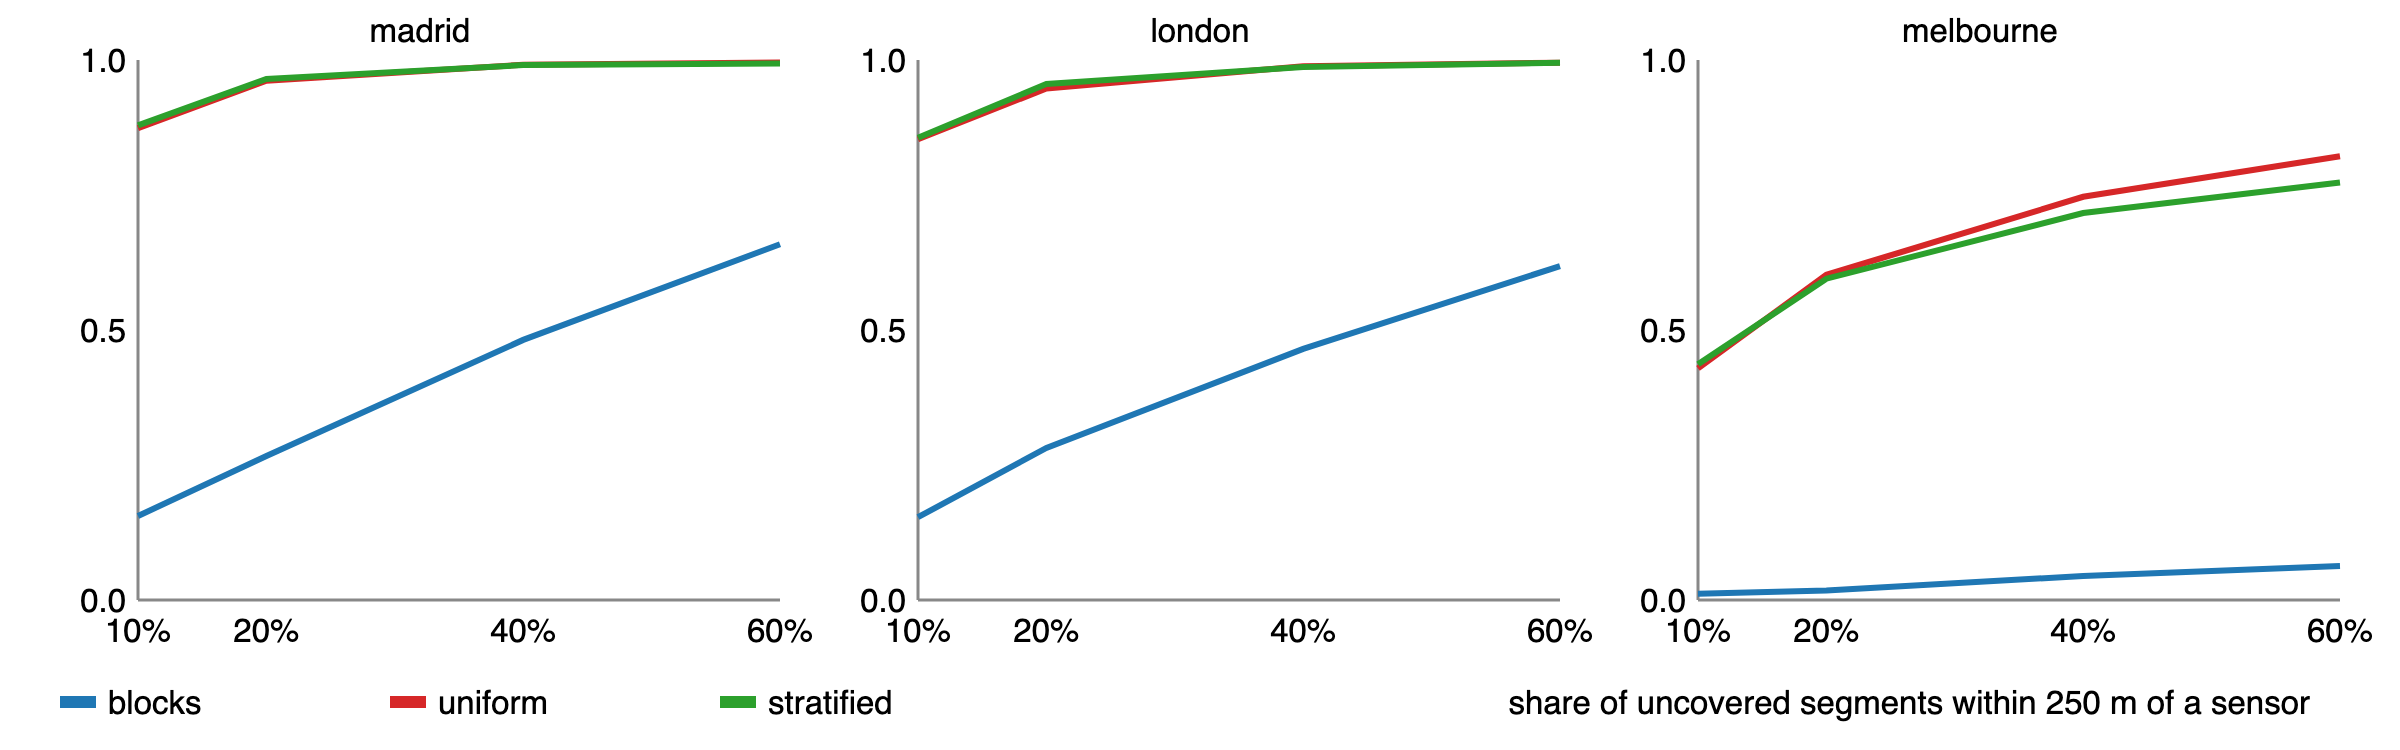
\includegraphics[width=\textwidth]{figures/e10geo_curva.png}
\caption{Share of uncovered segments with an instrumented segment within 250 m, against coverage. One panel per city; one line per rule (blocks, uniform, density-stratified); mean over 20 draws. Frozen figure \texttt{e10geo\_curva.svg} (a4edbde30583b455).}
\label{fig:e10geo}
\end{figure*}

\textbf{Placement changes proximity by a large factor.} Share of uncovered segments within 250 m of a sensor (mean over 20 draws, with the 2.5–97.5\% range):

\begin{table*}[!t]
\centering\footnotesize
\renewcommand{\arraystretch}{1.15}
\caption{E10-geo — how close can placement bring uncovered segments to a sensor?}
\begin{tabularx}{\textwidth}{>{\raggedright\arraybackslash\hsize=0.614\hsize}X>{\raggedright\arraybackslash\hsize=0.295\hsize}X>{\raggedright\arraybackslash\hsize=1.364\hsize}X>{\raggedright\arraybackslash\hsize=1.364\hsize}X>{\raggedright\arraybackslash\hsize=1.364\hsize}X}
\toprule
\textbf{City} & \textbf{\emph{f}} & \textbf{Blocks} & \textbf{Uniform} & \textbf{Density-stratified} \\
\midrule
Madrid & 10\% & 0.155 [0.078; 0.217] & 0.874 [0.785; 0.937] & 0.879 [0.810; 0.939] \\
Madrid & 20\% & 0.267 [0.149; 0.320] & 0.962 [0.936; 0.982] & 0.965 [0.953; 0.981] \\
Madrid & 40\% & 0.481 [0.315; 0.586] & 0.991 [0.985; 0.998] & 0.990 [0.979; 0.997] \\
Madrid & 60\% & 0.659 [0.453; 0.832] & 0.996 [0.991; 1.000] & 0.993 [0.983; 1.000] \\
London & 10\% & 0.153 [0.056; 0.225] & 0.853 [0.779; 0.929] & 0.856 [0.794; 0.929] \\
London & 20\% & 0.282 [0.199; 0.348] & 0.947 [0.917; 0.975] & 0.955 [0.929; 0.976] \\
London & 40\% & 0.465 [0.324; 0.603] & 0.988 [0.974; 0.997] & 0.987 [0.975; 0.996] \\
London & 60\% & 0.619 [0.493; 0.740] & 0.995 [0.989; 1.000] & 0.995 [0.986; 1.000] \\
Melbourne & 10\% & 0.012 [0.002; 0.023] & 0.429 [0.343; 0.494] & 0.436 [0.375; 0.515] \\
Melbourne & 20\% & 0.018 [0.003; 0.031] & 0.602 [0.558; 0.668] & 0.595 [0.563; 0.650] \\
Melbourne & 40\% & 0.044 [0.022; 0.081] & 0.746 [0.702; 0.771] & 0.717 [0.671; 0.749] \\
Melbourne & 60\% & 0.063 [0.027; 0.104] & 0.821 [0.757; 0.862] & 0.773 [0.739; 0.804] \\
\bottomrule
\end{tabularx}
\end{table*}

\textbf{Madrid and London.}

\begin{itemize}
\item At 10\% coverage, uniform placement puts 85–87\% of the uncovered segments within 250 m of a sensor. That is more than block placement reaches at 60\% (62–66\%).
\item The median distance from an uncovered segment to the nearest sensor falls from 775–786 m with blocks to 94–109 m with uniform placement.
\item From 20\% coverage, uniform placement brings at least 94.7\% of the uncovered segments within the radius.
\end{itemize}

\textbf{Melbourne.}

\begin{itemize}
\item Block placement leaves almost every uncovered segment beyond 250 m: 1–6\% are within it, with median distances of 1.2–4.2 km.
\item Uniform placement brings 43–82\% within 250 m.
\end{itemize}

\textbf{Oversampling sparse areas buys nothing in proximity.} The density-stratified rule matches the uniform one within 0.01 in Madrid and London. In Melbourne it is 3–5 points below it at 40–60\% coverage, because the sensors it moves to sparse areas leave the dense ones farther apart.

\begin{quote}
\textbf{At the same number of sensors, the placement rule decides whether one uncovered segment in seven or six in seven lies within 250 m of a sensor in Madrid and London. Between uniform and density-stratified placement there is no difference.}
\end{quote}

\textbf{What this proximity is worth.} E12-bis measured the value of a sensor within 250 m on the segments of E9. A calibrated predictor that uses it stays 1–3 points behind G0 in Madrid and London, and does not pass it. The label signal reached by placement therefore buys no forecast that the model without spatial exchange does not already give. E12-ter tests whether this still holds once the calendar is added to the neighbour.

\textbf{The answer to ``where''.} Placement decides where the network measures: which segments carry a sensor and which lie next to one. On these data it does not decide how well the segments without a sensor are forecast elsewhere. A placement rule is chosen for the segments it covers, not for what it predicts on the others.

\textbf{Limits stated with the result:}

\begin{itemize}
\item distances are straight-line between segment coordinates, not along the road;
\item the value of proximity comes from E12-bis on the block sets of E9, where the hidden segments within 250 m lie at the edges of corridors. That a hidden segment's value depends only on its distance to the nearest sensor, and not on the rule that placed the sensors, is an assumption, not a measurement;
\item 250 m is the radius found by E12 with its distance bins; the 500 m shares are in the frozen record.
\end{itemize}

% ---- section_discussion.md (297444621a421db8)
\section{Discussion}
\textbf{Why no further model.} One could object that the graph model of E9 is one model among many. A better architecture might extract what Graph WaveNet did not. The analyses without training answer this objection from the data rather than from the model.

\begin{itemize}
\item The calendar table of E12-ter uses the hour of the week of the target time and nothing else. It forecasts a segment without a sensor as well as the trained model without spatial exchange, in Madrid and London, and slightly better in Melbourne.
\item Adding the nearest instrumented neighbour's class to that table adds nothing within 250 m. Every interval there contains zero, and a 3-point gain is excluded.
\item Beyond 250 m, adding the neighbour makes the forecast worse.
\end{itemize}

A learned model can only exploit a dependence that the data contain. The dependence between a segment without a sensor and its neighbours, net of the calendar, is measured here as zero within the only radius where the labels agree. A second learned model would have to find a signal that neither the learned propagation (E9, E11) nor the calibrated tables (E12-bis, E12-ter) found. We therefore did not train one.

The argument has a stated perimeter. Two uses of the neighbours were tested:

\begin{itemize}
\item the calibrated class of a single neighbour (E12-bis, E12-ter);
\item a learned aggregation of several neighbours over three hours (G1 in E9).
\end{itemize}

Neither gained over the model without spatial exchange, on labels in three classes at 15–120 minutes. Continuous speeds, incidents and events were not tested.

\textbf{What the agreement of nearby labels is.} Two segments within 250 m share a class more often than chance. The natural reading is that congestion spreads along a corridor, so a sensor tells about its unmeasured neighbours. The forecasts say otherwise. Net of the hour of the week, the neighbour's class tells nothing about the segment's class 15 to 120 minutes later. Nearby segments agree because both are congested at the same hours of the same days. The calendar is common knowledge: it needs no sensor nearby.

\textbf{What placement can and cannot do.} The rule that chooses instrumented segments changes proximity by a large factor:

\begin{itemize}
\item contiguous blocks leave most uncovered segments far from any sensor;
\item uniform placement brings almost all of them within 250 m from 20\% coverage in Madrid and London, and 43–82\% in Melbourne;
\item density-stratified placement matches uniform placement.
\end{itemize}

If proximity had forecasting value, these differences would translate into accuracy. Since it has none beyond the calendar, the choice of placement should be made for the segments a sensor covers: where a measurement is needed for control, enforcement or detection. It should not be made for what the sensor might predict elsewhere.

\textbf{The operator's decision.} What a sensor buys is the measurement at its own segment. The question of what that measurement should be therefore becomes the main one, and it is the subject of Part A.

For the most common urban sensor, Part A gives a consistent answer. A loop detector says whether a segment is congested, not how congested it is: its reconstruction ranks levels poorly and separates congested cells almost perfectly, with a threshold that transfers between sensors. Its low agreement with probe speeds on arterials is about half a matter of matching a loop to a segment some 30 m away, so it says less about the loop than it seems. Per lane, detection is as good as on the ring; averaged over the lanes of a section, it loses the episodes that occur on one lane only, whatever the device. A target defined on the section mean therefore discards part of what the sensor measures. The definition of the target matters as much as the device.

\textbf{Relation to propagation results in the literature.} Graph models for traffic are usually evaluated on sensors whose own history is in training or in the input [wu2019gwnet]. Kriging methods estimate unobserved locations from simultaneous observations, not forecasts at 15–120 minutes [wu2021ignnk]. The deliverable that preceded this work found propagation gains with hidden segments that were training targets. Our positive control reproduces that condition and the gain that comes with it. Our negative result does not contradict those findings: it concerns a stricter regime, the one an operator faces for a segment that has never had a sensor. [ref: placement and coverage studies, to be chosen.]

% ---- section_limits.md (e319de6a2db17c62)
\section{Limits}
\textbf{Task and data.}

\begin{itemize}
\item One task: three congestion classes, 15–120 minutes ahead, from measured speeds of three Traffic4cast cities. Other targets (speed, travel time), longer horizons and other data sources are not tested.
\item The cities' series are one-week blocks separated by gaps; only origins whose window and targets respect the 15-minute cadence are used (register of corrections, item 1).
\item The classes come from a congestion factor relative to free flow, with thresholds inherited from the deliverable.
\end{itemize}

\textbf{Models.}

\begin{itemize}
\item One architecture, Graph WaveNet, with and without its graph, inherited and not tuned. The training budget is fixed by a pilot (1,000 updates) and checked at twice that budget.
\item No static attribute of the segments (number of lanes, capacity, speed limit). In Madrid and London these attributes are missing, and in the E11 pilot the speed limit acted as an identifier of the node.
\item The training input covers 60–95\% of the observed set, while evaluation uses all of it. The shift is the same at every coverage.
\end{itemize}

\textbf{Design.}

\begin{itemize}
\item Hidden segments are drawn as whole blocks of a grid. At 60\% coverage the test-hidden segments lie in 8–9 blocks, and in Melbourne the intervals are wide.
\item In Melbourne the 0–250 m bin of the analyses without training is empty or has too few blocks at every coverage. The statements of E12-bis and E12-ter are ``undetermined'' for that reason alone.
\item The 3-point margin is a convention, inherited from the earlier study. No correction for multiple comparisons is applied; this is declared in each pre-registration.
\end{itemize}

\textbf{The analyses without training.}

\begin{itemize}
\item \textbf{Perimeter of the negative result.} Two ways of using the neighbours were tested, and neither gained over the model without spatial exchange:
\begin{itemize}
\item the calibrated class of a single neighbour (E12-bis, E12-ter);
\item a learned aggregation of several neighbours over three hours (G1, E9).
\end{itemize}
\par  Both concern labels in three classes at 15–120 minutes. Continuous speeds, incidents and events were not tested.
\item The calendar is the hour of the week. Holidays and events are not modelled.
\item The agreement of nearby labels was measured at the same instant, and its value net of the calendar was measured as a forecast at 15–120 minutes. The reading ``shared calendar'' is a reading of the forecasts, not a decomposition of the same-instant agreement.
\item Distances are straight-line between segment coordinates, not along the road.
\end{itemize}

\textbf{Placement.}

\begin{itemize}
\item The value of proximity was measured on the block placements of E9. That a hidden segment's value depends only on its distance to the nearest sensor, and not on the rule that placed the sensors, is an assumption.
\item Placement rules that use traffic data (for example, instrumenting the most congested segments) are not compared. With no forecasting value in proximity, they could only change which segments are measured.
\end{itemize}

\textbf{Part A.}

\begin{itemize}
\item The three datasets do not overlap in time or space. Regime and technology cannot be separated: the ring is observed in 2024, the arterials in 2021.
\item The reading rules were fixed knowing the deliverable's in-sample values, so every statement of Part A is descriptive.
\item The free-flow references use the whole year, as built in the deliverable's targets. Part A compares measurements; it does not forecast.
\item The 19–72 m band was built a posteriori by the deliverable, and the matching share depends on it.
\item Austin has 6 three-lane and 2 four-lane sections; no lane threshold is identified.
\item Several printed values of the deliverable have no conserved generator (register of corrections, items 14–20). They are reported as such; every number of Part A is regenerated.
\end{itemize}

\textbf{Reproducibility.} Costs are measured on one machine (Mac M3 Max); the campaign times are from concurrent processes and are not isolated costs. The regeneration script reruns every analysis from the per-cell predictions; it does not retrain the models.

% ---- section_conclusion.md (c41ec8a744e6f4a9)
\section{Conclusion}
We asked what an operator can buy with traffic sensors for the segments of the network that have none. Every experiment was pre-registered and frozen, on three cities, at 15–120 minutes.

On segments without a sensor, these data carry no forecastable spatial information beyond the calendar:

\begin{itemize}
\item a learned graph model gains nothing over the same model without its graph, at any spacing and any coverage tested;
\item the labels of nearby segments agree, but only within about 250 m;
\item calibrated, that agreement does not beat the model without spatial exchange;
\item net of the hour of the week, it is worth nothing.
\end{itemize}

Placement decides how many uncovered segments lie near a sensor: in Madrid and London at 10\% coverage, one in seven with contiguous blocks and six in seven with uniform placement. It does not decide how well they are forecast.

What a sensor buys is the measurement at its own segment. The choice that matters is therefore what to measure. For the loop detector, Part A finds that:

\begin{itemize}
\item it measures the occurrence of congestion rather than its level, with a threshold that transfers between sensors;
\item about half of its disagreement with probe speeds on arterials comes from matching it to a segment some 30 m away;
\item averaging its lanes hides the episodes that occur on one of them.
\end{itemize}

Two directions remain open:

\begin{itemize}
\item inputs that neither the models nor the tables had: speeds rather than classes, incidents, events;
\item the same inductive regime on other networks and other measurement technologies.
\end{itemize}

The pre-registrations, frozen records, per-cell predictions and the script that regenerates every number are released with the paper.

\clearpage
\onecolumn
\appendices
\renewcommand{\thesection}{S\arabic{section}}
\section*{Supplementary material: register of corrections}
\addcontentsline{toc}{section}{Supplementary material}
Source: \texttt{protocol/\allowbreak{}paper4/\allowbreak{}REGISTRO\_\allowbreak{}CORREZIONI.\allowbreak{}md} (979bb29cb58be054). The main text refers to these items by number.

Consolidated list of the defects found during Paper 4, with the correction adopted and its source. Items 1–3 are defects of the deliverable UC-04 pipeline found during Phase 0 and the drafting of the protocol; they are corrected in the Paper 4 pipeline, not in the deliverable. Item 7 is a defect of the deliverable's negative control, found while drafting E11; item 8 is a defect of the Paper 4 pipeline (the E11 generator), corrected before any output. Items 9–13 are defects of the Paper 4 pipeline, records or measurements found during Part B; none changed a number accepted by the internal review (register completed on 2026-11-08, after Part B was closed). Items 14–17 are defects of the deliverable found while drafting the pre-registration of Part A (\texttt{protocol/\allowbreak{}paper4/\allowbreak{}P4A.\allowbreak{}md}). They have no effect on the numbers of the paper, which are all regenerated. Items 18–20 are discrepancies between the deliverable's printed tables and the regenerated ones, found by the comparison in \texttt{CONGELAMENTO\_\allowbreak{}4A.\allowbreak{}md} (a0b76dc). In each case the conserved script, run on the fingerprinted inputs, prints the regenerated values (\texttt{paper4/\allowbreak{}runs/\allowbreak{}p4a/\allowbreak{}script\_\allowbreak{}*.\allowbreak{}txt}), so the deliverable's tables came from another version of the script or of its inputs. Their causes were measured by the executor, read-only, with the deliverable's conserved module (\texttt{analisi/\allowbreak{}p4a\_\allowbreak{}cause.\allowbreak{}py}, \texttt{protocol/\allowbreak{}paper4/\allowbreak{}fase2/\allowbreak{}CAUSE\_\allowbreak{}4A.\allowbreak{}md}, commit 03fd226): one is found (item 18, green class), the rest have no conserved generator. No number of the paper changes; the frozen record carries a dated note at its end. Items 4–6 are defects of traceability of the deliverable found in Phase 1 (questions D7–D9 of \texttt{paper4/\allowbreak{}DOMANDE.\allowbreak{}md}): register only, no Paper 4 number depends on them. The paper refers to the items by number.

Other defects of the deliverable found in Phase 0 are listed in \texttt{paper4/\allowbreak{}RICOGNIZIONE.\allowbreak{}md} §0, but are not registered here because no Paper 4 number depends on them:

\begin{itemize}
\item the randomisation preserved only the edge count;
\item hidden nodes entered the loss;
\item the resampling used \texttt{np.\allowbreak{}isin}.
\end{itemize}

{\scriptsize
\begin{longtable}{>{\raggedright\arraybackslash}p{0.03\textwidth}>{\raggedright\arraybackslash}p{0.27\textwidth}>{\raggedright\arraybackslash}p{0.38\textwidth}>{\raggedright\arraybackslash}p{0.11\textwidth}>{\raggedright\arraybackslash}p{0.13\textwidth}}
\toprule
\textbf{\#} & \textbf{Defect} & \textbf{Correction and measured effect} & \textbf{Found by} & \textbf{Source} \\
\midrule
\endhead
1 & Windows built by index across calendar jumps: the Traffic4cast series are one-week blocks separated by 7-day jumps (Madrid 15, London 16, Melbourne 15), and \texttt{models/\allowbreak{}gomo\_\allowbreak{}sparse.\allowbreak{}py:119} builds origins as \texttt{arange} over raw indices & admissible-origin rule (15-min cadence from the first input step to the last target), with a causality test, as in Paper 1 (register of corrections item 5). Effect: to be measured as the share of excluded origins per city & reading the timestamps of the target files while drafting the perimeter, 2026-11-06 & \texttt{protocol/\allowbreak{}paper4/\allowbreak{}PROTOCOLLO.\allowbreak{}md} §2.3 \\ \addlinespace
2 & Free-flow reference on the loop contexts computed as the 85th percentile of speed over the whole year, test period included (\texttt{OR3/\allowbreak{}data\_\allowbreak{}collection/\allowbreak{}go-\allowbreak{}mo/\allowbreak{}2\_\allowbreak{}gomo\_\allowbreak{}targets.\allowbreak{}py:42}) & 85th percentile on the training period only, if GO-MO contexts are used in forecasting; the city contexts use the provider's \texttt{free\_\allowbreak{}flow\_\allowbreak{}kph}, which is causal & reading the target builders, 2026-11-06 & \texttt{protocol/\allowbreak{}paper4/\allowbreak{}PROTOCOLLO.\allowbreak{}md} §2.1 \\ \addlinespace
3 & Population: \texttt{gomo\_\allowbreak{}sparse.\allowbreak{}py} aligns 828 / 774 / 587 nodes (Madrid, London, Melbourne), not the 900 / 900 / 594 of the target files & declared; the same difference as Paper 1, register of corrections item 8 & \texttt{aligned graph} lines in \texttt{OLD/\allowbreak{}log/\allowbreak{}sparse\_\allowbreak{}5semi.\allowbreak{}log}, \texttt{sparse\_\allowbreak{}fixed.\allowbreak{}log}, \texttt{gomo\_\allowbreak{}corretto.\allowbreak{}log}, 2026-11-06 & \texttt{protocol/\allowbreak{}paper4/\allowbreak{}PROTOCOLLO.\allowbreak{}md} §2.3 \\ \addlinespace
4 & Tables 34-35 (negative control of the geometry) could be regenerated only after fixing the pairing in the conserved script: \texttt{analisi/\allowbreak{}geometria\_\allowbreak{}criteri.\allowbreak{}py} paired the true and randomised graphs by looking for \texttt{knn} in the graph \emph{name} (r. 202-203), whereas \texttt{knn} is the \texttt{modo} column and the names are \texttt{comp\_\allowbreak{}q\textless{}xy\textgreater{}} / \texttt{neg\_\allowbreak{}rand\_\allowbreak{}q\textless{}xy\textgreater{}} (\texttt{make\_\allowbreak{}geo\_\allowbreak{}sweep.\allowbreak{}py} r. 52, 76); the result CSVs are also named \texttt{geo\_\allowbreak{}\textless{}city\textgreater{}\_\allowbreak{}\textless{}graph\textgreater{}\_\allowbreak{}s\textless{}s\textgreater{}.\allowbreak{}csv} while the script looked for \texttt{geo\_\allowbreak{}\textless{}graph\textgreater{}\_\allowbreak{}s\textless{}s\textgreater{}.\allowbreak{}csv} (r. 142, 206-207). No pair was ever found with the preserved script; the tables were nevertheless computed from the preserved CSVs, since the re-run reproduces them exactly & pairing by \texttt{comp\_\allowbreak{}q\textless{}xy\textgreater{}} $\leftrightarrow$ \texttt{neg\_\allowbreak{}rand\_\allowbreak{}q\textless{}xy\textgreater{}} of the same city and city-prefixed CSV names (\texttt{evoluzione/\allowbreak{}audit/\allowbreak{}patch/\allowbreak{}patch\_\allowbreak{}p4\_\allowbreak{}criterio4.\allowbreak{}py}, 2026-11-06); criterion 4 re-run on the preserved CSVs (\texttt{OLD/\allowbreak{}replication/\allowbreak{}geo/\allowbreak{}}, 5 seeds), row-by-row comparison with Tables 34-35 in \texttt{protocol/\allowbreak{}paper4/\allowbreak{}fase1/\allowbreak{}GEOMETRIA\_\allowbreak{}CRITERIO4\_\allowbreak{}rigenerato.\allowbreak{}md}: Tables 34-35 and the Melbourne run (text, p. 96) reproduced exactly, including the per-seed values. Register only: no Paper 4 number depends on it & search for the generator of Tables 34-35 (D7), 2026-11-06 & \texttt{protocol/\allowbreak{}paper4/\allowbreak{}fase1/\allowbreak{}GEOMETRIA\_\allowbreak{}CRITERIO4\_\allowbreak{}rigenerato.\allowbreak{}md} \\ \addlinespace
5 & Table 66 (ratio between the rank correlation of the raw inputs and that of the reconstructed factor) has no generator: \texttt{data\_\allowbreak{}collection/\allowbreak{}t4c\_\allowbreak{}crossval.\allowbreak{}py} prints the per-input correlations to the screen (r. 137-160) and saves only the pairs (r. 194); no script computes the ratio. The \texttt{-\allowbreak{}-\allowbreak{}exclude-\allowbreak{}empty} and \texttt{-\allowbreak{}-\allowbreak{}max-\allowbreak{}dist 30} outputs (README §7.11, r. 727-729) were not preserved & the three README commands re-run with preserved outputs, fingerprints of CSVs and inputs, comparison with Tables 64-65 in \texttt{protocol/\allowbreak{}paper4/\allowbreak{}fase1/\allowbreak{}CROSSVAL\_\allowbreak{}rigenerato.\allowbreak{}md} (Tables 64-65 and the 30 m sensitivity reproduced exactly; base CSV byte-identical to the preserved one); Table 66 not regenerated (no generator), to be recomputed from the preserved screen outputs if needed & search for the generator of Tables 64-66 (D8), 2026-11-06 & \texttt{protocol/\allowbreak{}paper4/\allowbreak{}fase1/\allowbreak{}CROSSVAL\_\allowbreak{}rigenerato.\allowbreak{}md} \\ \addlinespace
6 & \texttt{t4cmad\_\allowbreak{}rand\_\allowbreak{}k1.\allowbreak{}pkl}, \texttt{t4cmad\_\allowbreak{}rand\_\allowbreak{}k2.\allowbreak{}pkl} (written in the same second, 22/8/2026) and \texttt{t4cmad\_\allowbreak{}identity\_\allowbreak{}graph.\allowbreak{}pkl} (21/8/2026) have no generator in the repository, in the untracked files or in the two histories; the only traces of use are \texttt{OLD/\allowbreak{}log/\allowbreak{}randk.\allowbreak{}log} (ten runs of \texttt{models/\allowbreak{}gomo\_\allowbreak{}sparse.\allowbreak{}py} whose CSVs \texttt{replication/\allowbreak{}randk\{1,2\}\_\allowbreak{}t4cmad\_\allowbreak{}s\{0-\allowbreak{}4\}.\allowbreak{}csv} were not preserved) and \texttt{OLD/\allowbreak{}log/\allowbreak{}identita.\allowbreak{}log} (\texttt{replication/\allowbreak{}identita/\allowbreak{}ident\_\allowbreak{}t4cmad\_\allowbreak{}s0-\allowbreak{}4.\allowbreak{}csv}, preserved) & graphs characterised from the files (nodes, edges, degree distribution, weights, overlap with the road graph, fingerprints) in \texttt{protocol/\allowbreak{}paper4/\allowbreak{}fase1/\allowbreak{}GRAFI\_\allowbreak{}SENZA\_\allowbreak{}GENERATORE.\allowbreak{}md}; no result of the deliverable is traced to them & search for the generator (D9), 2026-11-06 & \texttt{protocol/\allowbreak{}paper4/\allowbreak{}fase1/\allowbreak{}GRAFI\_\allowbreak{}SENZA\_\allowbreak{}GENERATORE.\allowbreak{}md} \\ \addlinespace
7 & Negative control of the deliverable's geometry: the randomised edges carried their new geographic distance as weight (\texttt{make\_\allowbreak{}geo\_\allowbreak{}sweep.\allowbreak{}py:49}, \texttt{weight = D[a, b] + 1}) with a kernel $\sigma$ of their own (\texttt{models/\allowbreak{}gomo\_\allowbreak{}sparse.\allowbreak{}py:149}); on the three preserved pairs the mean kernel was 0.23–0.36 for the randomised graphs against 0.20–0.48 for the kNN graphs, with randomised medians 0.04–0.26, and the three randomised graphs were not connected. Weights, topology and connectivity differed together: the control did not isolate the geometry & E11: both randomised graphs receive the multiset of G1's weights permuted over their edges, and connectivity is preserved (\texttt{protocol/\allowbreak{}paper4/\allowbreak{}E11.\allowbreak{}md}, Design, preflight 5 and 5-bis). Register only: no Paper 4 number depends on the deliverable's control & weight check on \texttt{geo\_\allowbreak{}sweep/\allowbreak{}*\_\allowbreak{}neg\_\allowbreak{}rand\_\allowbreak{}*.\allowbreak{}pkl} against the kNN pairs, 2026-11-06 & \texttt{protocol/\allowbreak{}paper4/\allowbreak{}E11.\allowbreak{}md} \\ \addlinespace
8 & Defect of the E11 frozen-record generator: the red-recall step indexed \texttt{p[:, nodes, :, 2]} in one step, which numpy reorders to (nodes, origins, horizons); the first run stopped with an IndexError (14 against 997) before writing any output & node and class selected in two steps (\texttt{red\_\allowbreak{}recall} in \texttt{paper4/\allowbreak{}code/\allowbreak{}genera\_\allowbreak{}congelamento\_\allowbreak{}e11.\allowbreak{}py}, commit b2863c9); recall added to the self-test with origins $\neq$ nodes, and an end-to-end self-test on a synthetic copy of the campaign. No number was produced by the defective version & first run of the generator by the executor, 2026-11-06 & \texttt{paper4/\allowbreak{}congelamenti/\allowbreak{}CONGELAMENTO\_\allowbreak{}E11.\allowbreak{}md}, deviations item 7 \\ \addlinespace
9 & First E11 node-set rule: on three Melbourne pairs (configuration $\times$ seed) the realised shares of observed, validation-hidden and test-hidden nodes fell outside $\pm$15 points of the targets; the preflight reported 22 of 23 checks passed & cells assigned by deficit on the target shares 40/20/40, on the smallest grid G $\geq$ 6 with at least 20 occupied cells; geometry covariates registered with the node sets; preflight 4-bis passed on all 12 configurations $\times$ 5 seeds. Found and corrected before any training & E11 preflight, 2026-11-06 (commit e363bf7; correction 21db33d) & \texttt{protocol/\allowbreak{}paper4/\allowbreak{}E11.\allowbreak{}md}, Design and preflight 4-bis \\ \addlinespace
10 & The first E11 frozen record reported red recall at the 5\% false-alarm threshold chosen on validation without the false-alarm rate realised on test, so a recall could be read as discrimination where the threshold was not met & the generator reports the realised rate next to every recall (commit 5cda9c3); record regenerated with every number identical to the previous one (\texttt{-\allowbreak{}-\allowbreak{}compare-\allowbreak{}with}; 4e04ba7, 459b43ee3e649a31). The same rule holds in E9, E12, E12-bis and E12-ter & drafting of the E11 section, 2026-11-06 & \texttt{paper4/\allowbreak{}congelamenti/\allowbreak{}CONGELAMENTO\_\allowbreak{}E11.\allowbreak{}md} \\ \addlinespace
11 & The first two isolated cost measurements of G1-rand(deg) in E9 ran during Spotlight indexing (load average 36–62) and gave 303.8 s and 393.9 s against 159–179 s for G1 & arm re-measured alone with Spotlight idle (135.9 s), and G1 in the same conditions (168.5 s); the signature line reports these; the earlier figures stay in the manifest, unused & the executor, cost measurement, 2026-11-07 & \texttt{protocol/\allowbreak{}paper4/\allowbreak{}E9.\allowbreak{}md}, Deviations 1 \\ \addlinespace
12 & The first synthetic self-test of E12-bis populated only the 0–250 m bin, so its condition ``beats the prior more strongly within 250 m than in the outer bins'' was met vacuously & synthetic world widened (clusters across 20 km) and at least one outer bin required (\texttt{selftest} in \texttt{paper4/\allowbreak{}code/\allowbreak{}e12bis.\allowbreak{}py}); found and corrected before the preflight and the signature & drafting of the E12-bis code, 2026-11-08 & \texttt{paper4/\allowbreak{}code/\allowbreak{}e12bis.\allowbreak{}py} (27adfe03f24647e8) \\ \addlinespace
13 & The frozen E12 code (\texttt{e12.\allowbreak{}py}, 3ec453d15372b217) had no input check after the run and no end-to-end self-test of its frozen-record generator, which E9 and E11 had & both added outside the frozen file, in \texttt{paper4/\allowbreak{}code/\allowbreak{}verifica\_\allowbreak{}e12.\allowbreak{}py} (e4b753bc52fdf7f5, commit ac545db), before the campaign; E12-bis and E12-ter carry them inside their own code & drafting of the E12 commands for the executor, 2026-11-08 & \texttt{paper4/\allowbreak{}code/\allowbreak{}verifica\_\allowbreak{}e12.\allowbreak{}py} \\ \addlinespace
14 & The area under the curve on the Madrid arterials, 0.542 (Table 68, p. 132; text p. 131; Gini 0.084), and with it the 58\% / 42\% split of the arterial gap (p. 132), has no source: it is hard-coded at line 195 of \texttt{analisi/\allowbreak{}validazione\_\allowbreak{}colocalizzata.\allowbreak{}py}, and no script, log or output in \texttt{OR3/\allowbreak{}} or \texttt{OLD/\allowbreak{}} contains it & recomputed in Part A from the 399 base pairs of \texttt{t4c\_\allowbreak{}crossval.\allowbreak{}py}: median over pairs of the per-pair area under the curve (primary) and value on the pooled cells (secondary), with intervals; the split recomputed from them. Defect of the deliverable; no effect on the numbers of the paper, which are all regenerated & search of \texttt{OR3/\allowbreak{}} and \texttt{OLD/\allowbreak{}} while drafting P4A, 2026-11-08 & \texttt{protocol/\allowbreak{}paper4/\allowbreak{}P4A.\allowbreak{}md}, Design, step 0 \\ \addlinespace
15 & The rank correlation on the Madrid arterials is +0.001 in Table 68 (p. 132, hard-coded at line 195 of the same script) and +0.071 in the text of p. 131 and in the script's docstring: two values for the same quantity, neither computed & recomputed in Part A in the same two ways as item 14; both deliverable values reported next to the recomputed ones. Defect of the deliverable; no effect on the numbers of the paper & reading of Table 68 against the text, 2026-11-08 & \texttt{protocol/\allowbreak{}paper4/\allowbreak{}P4A.\allowbreak{}md}, Design, step 0 \\ \addlinespace
16 & The Austin volume–occupancy rank correlations at lane and at section level, +0.7241 and +0.2999 (text p. 133), have no generator: no line of \texttt{analisi/\allowbreak{}validazione\_\allowbreak{}colocalizzata.\allowbreak{}py} computes them & recomputed in Part A from the Austin data with a declared definition (sections with at least 3 lanes, after the script's filters). Defect of the deliverable; no effect on the numbers of the paper & reading of the script against the text, 2026-11-08 & \texttt{protocol/\allowbreak{}paper4/\allowbreak{}P4A.\allowbreak{}md}, Design, step 0 \\ \addlinespace
17 & The within-lane area under the curve in Austin, ``0,990, con intervallo [0,959; 0,999]'' (text p. 131), presents as an interval the interquartile range across lanes printed by the script; the brackets of Table 69 are also interquartile ranges & reported in Part A as interquartile ranges, with the bootstrap interval over sections next to them (correction 2). Defect of the deliverable; no effect on the numbers of the paper & reading of \texttt{sez\_\allowbreak{}austin} against the text, 2026-11-08 & \texttt{protocol/\allowbreak{}paper4/\allowbreak{}P4A.\allowbreak{}md}, Correction 2 \\ \addlinespace
18 & Table 67, measured class green: the deliverable counts 2,989,877 cells and a rank correlation of +0.033; the regenerated table counts 3,432,842 and +0.012, and its three classes sum to the 4,199,040 non-imputed cells while the deliverable's do not. The overall rank correlation is +0.255 printed against +0.249 regenerated. The other rows of Table 67 are identical & cause (executor, 2026-11-08): the deliverable's green class was 0.8 $\leq$ r\_tr \textless{} 1.5. The 442,965 cells it misses are exactly those whose measured factor is clipped at 1.5 (\texttt{carica\_\allowbreak{}m30}); with that class the conserved module gives 2,989,877 cells and +0.0326. The conserved code has 1.6 (\texttt{validazione\_\allowbreak{}colocalizzata.\allowbreak{}py}, line 117) in its only commit (dc8b6bb, 2026-09-17), so the version that printed the table is not conserved. The overall +0.255 is reproduced neither by that class nor by six other cell sets (+0.249 to +0.480): generator not found. Defect of the deliverable; no effect on the numbers of the paper & comparison in \texttt{CONGELAMENTO\_\allowbreak{}4A.\allowbreak{}md}; causes in \texttt{CAUSE\_\allowbreak{}4A.\allowbreak{}md} (03fd226), 2026-11-08 & \texttt{paper4/\allowbreak{}congelamenti/\allowbreak{}CONGELAMENTO\_\allowbreak{}4A.\allowbreak{}md}, comparison and dated note; \texttt{protocol/\allowbreak{}paper4/\allowbreak{}fase2/\allowbreak{}CAUSE\_\allowbreak{}4A.\allowbreak{}md} \\ \addlinespace
19 & Table 68, neighbour bands: rank correlation, area under the curve and Gini differ from the deliverable by 0.001–0.009; median distances identical (14 / 31 / 31 / 96 m). Regenerated sensors per band: 191 / 181 / 156 / 165 & cause (executor, 2026-11-08): the deliverable's table does not print sensors per band; the filter of \texttt{p4a.\allowbreak{}py} is the conserved one (\texttt{sez\_\allowbreak{}accoppiamento}, lines 176–178), so the counts are those of that filter. Not caused by the coordinate file (\texttt{traffic\_\allowbreak{}sensors.\allowbreak{}csv} and \texttt{traffic\_\allowbreak{}sensors\_\allowbreak{}lug2026.\allowbreak{}csv} give the same rows). No variant of the cell filter reproduces the differences: without the imputation filter on the loop and with a positive loop speed the values are identical to ours; the nearest neighbour and the exclusion of the clipped cells of item 18 move further away. Not found; version not conserved. Defect of the deliverable; no effect on the numbers of the paper & comparison in \texttt{CONGELAMENTO\_\allowbreak{}4A.\allowbreak{}md}; causes in \texttt{CAUSE\_\allowbreak{}4A.\allowbreak{}md} (03fd226), 2026-11-08 & \texttt{paper4/\allowbreak{}congelamenti/\allowbreak{}CONGELAMENTO\_\allowbreak{}4A.\allowbreak{}md}, comparison and dated note; \texttt{protocol/\allowbreak{}paper4/\allowbreak{}fase2/\allowbreak{}CAUSE\_\allowbreak{}4A.\allowbreak{}md} \\ \addlinespace
20 & Austin sections: the brief counts 31; after the script's filters there are 40 (10 with one lane, 30 with at least 2: 22 / 6 / 2, as in Table 69); correction 3 uses 29. The deliverable states a lane–AUC rank correlation of −0.541 (p = 0.002) over 31 sections and excludes one section for a prevalence difference of −45.1 points. The prevalence differences of 3 and 4 lanes are +18.62 and +9.88 points, against +18.35 and +9.93 printed & cause (executor, 2026-11-08): the 40 sections are \texttt{intname|\allowbreak{}direction} after excluding the three intersections without direction. The only definition that gives 31 is ``sections with a defined area under the curve (more than 20 congested and more than 20 non-congested cells), whatever the number of lanes'': the 29 plus 2 with one lane. The section that leaves correction 3 is \texttt{LAMARZENNIA|\allowbreak{}SB}: 2 lanes, 43,081 aggregated cells, 11 with a congested lane, so its area under the curve is undefined. The −0.541 is not reproduced (−0.269, p = 0.144, over those 31; −0.441, p = 0.017, over the 29), and no conserved script computes it. The section at −45.1 points does not exist under the conserved code: every prevalence difference is $\geq$ 0 by construction (maximum +52.0, \texttt{BurnetRutland|\allowbreak{}SB}). Generator not found for either; the two prevalence differences are not traced. Defect of the deliverable; no effect on the numbers of the paper & comparison in \texttt{CONGELAMENTO\_\allowbreak{}4A.\allowbreak{}md} and preflight count; causes in \texttt{CAUSE\_\allowbreak{}4A.\allowbreak{}md} (03fd226), 2026-11-08 & \texttt{paper4/\allowbreak{}congelamenti/\allowbreak{}CONGELAMENTO\_\allowbreak{}4A.\allowbreak{}md}, comparison and dated note; \texttt{protocol/\allowbreak{}paper4/\allowbreak{}fase2/\allowbreak{}CAUSE\_\allowbreak{}4A.\allowbreak{}md}; \texttt{protocol/\allowbreak{}paper4/\allowbreak{}P4A.\allowbreak{}md}, Correction 3 \\ \addlinespace
\bottomrule
\end{longtable}
}
\end{document}
